\documentclass[12pt,a4paper]{report}
\usepackage[utf8]{inputenc}
\usepackage{amsmath}
\usepackage{amsfonts}
\usepackage{amssymb}
\usepackage{graphicx}
\usepackage{caption}
\usepackage{svg}
%\usepackage{gensymb}
\usepackage{fourier}
\usepackage[francais]{babel}
\usepackage{eurosym}

\usepackage[top=2.5cm,bottom=2.5cm,right=2.5cm,left=2.5cm]{geometry}

\usepackage{url}
\usepackage{moreverb}
%\usepackage{multirow}
%\author{LEJEUNE Raphaël}
%\title{Titre}

\usepackage[fpms]{umons-coverpage}
\umonsAuthor{Raphaël \textsc{LEJEUNE} \\ Maximilien \textsc{POTTIEZ}}
\umonsTitle{Un robot contrôlé via un Raspberry Pi}
\umonsSubtitle{Projet d'informatique}
\umonsDocumentType{Rapport de projet}
\umonsSupervisor{Sous la direction de Monsieur le Professeur\\ Mohammed \textsc{BENJELLOUN}}
\umonsDate{2015}

\begin{document}

\umonsCoverPage

\tableofcontents

\chapter{Introduction}

Nous avons imaginé le concept de \textbf{BotCop}, car la sécurité est devenu un thème central pour les habitations modernes. En effet, 75.000 cambriolages ont eu lieu en 2012 et en 2013 en Belgique \footnote{Source : \url{https://www.besafe.be/fr/diw/belgi-belgique}, visité le 13 août 2015}.

Bien que de plus en plus d'habitations soient équipées de systèmes de surveillance électronique, ceux-ci ne sont pas toujours fiables. Ces systèmes sont généralement basés sur des capteurs de température et de mouvements, et peuvent se déclencher sans raison en été, lorsque les températures sont hautes.

Les systèmes de surveillance avec caméra sont très couteux. Notre projet permettrait, en complément avec un système meilleur marché, d'obtenir des images en temps réel de la maison.

Installer une caméra fixe n'est pas très utile, à moins de n'avoir qu'une seule pièce à surveiller. Il faut donc pouvoir déplacer cette caméra. Voilà donc pourquoi nous avons voulu créer un robot.

Concrètement, BotCop pourra se déplacer dans toute la maison et renvoyer l'image filmée par sa caméra à l'utilisateur.

L'utilisateur pourra donc :

\bigbreak
\begin{itemize}
\item Contrôler le robot pour le déplacer,
\item Contrôler la caméra, pour pouvoir regarder partout dans n'importe quelle direction,
\item Visionner graphiquement le trajet vu du dessus dans l'interface
\end{itemize}

\newpage

We imagined the \textbf{BotCop} concept, because security became a central theme for modern houses. Actually, 75.000 burglaries occurred in 2012 and in 2013 in Belgium \footnote{From \url{https://www.besafe.be/fr/diw/belgi-belgique}, visited on 13 august 2015}.

Although more and more houses are equipped with electronic surveillance system, the latter are not always reliable. These systems usually are based on heat and movement sensors, and those can be triggered with no reason in the summer, when the temperatures are high.

Camera based surveillance systems are expensive. Our project would allow to get an image from the house in real time, with a cheaper system.

Set up a fixed camera is useless, unless there is only one room to monitor. This is why we need a mobile camera, and this is why we wanted to create a robot.

Concretely, BotCop can move in the house, and send the image back to the user.

The user will get the possiblity to :

\bigbreak
\begin{itemize}
\item Control the robot to move it,
\item Control the camera, to look everywhere in any direction,
\item See a graphic representation of the path followed by the robot.
\end{itemize}

%\begin{figure}[hf!]
%\center
%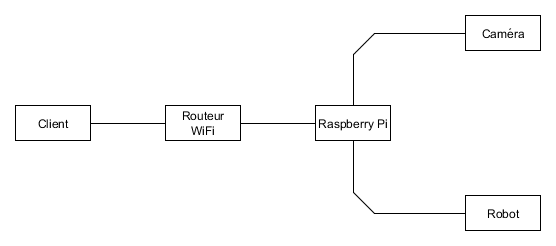
\includegraphics[scale=0.6]{images/GraphMateriel.png}
%\caption{Matériel}
%\end{figure}

\chapter{Matériel} \label{Matériel}

\begin{figure}[hf!]
\center
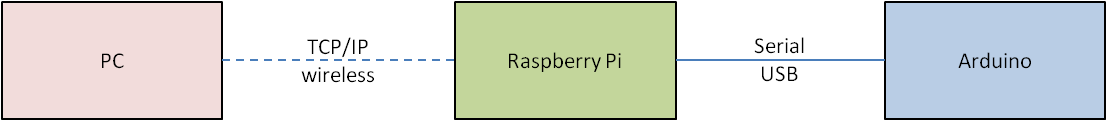
\includegraphics[scale=0.8]{images/ArchitectureMaterielle.png}
\caption{Architecture matérielle, et types de communication}
\end{figure}

Voici la liste complète du matériel que nous avons utilisé :

\paragraph{Kit} Le kit que nous utilisons se compose des éléments suivants :

\begin{itemize}
\item Chassis Bundle
\item Raspberry pi 2
\item Arduino
\item Batterie : TeckNet iEP387
\item Carte micro SD
\item Raspberry pi camera
\item Wifi : Edimax EW-7811Un -150Mbps
\end{itemize}

\begin{figure}[hf!]
\center
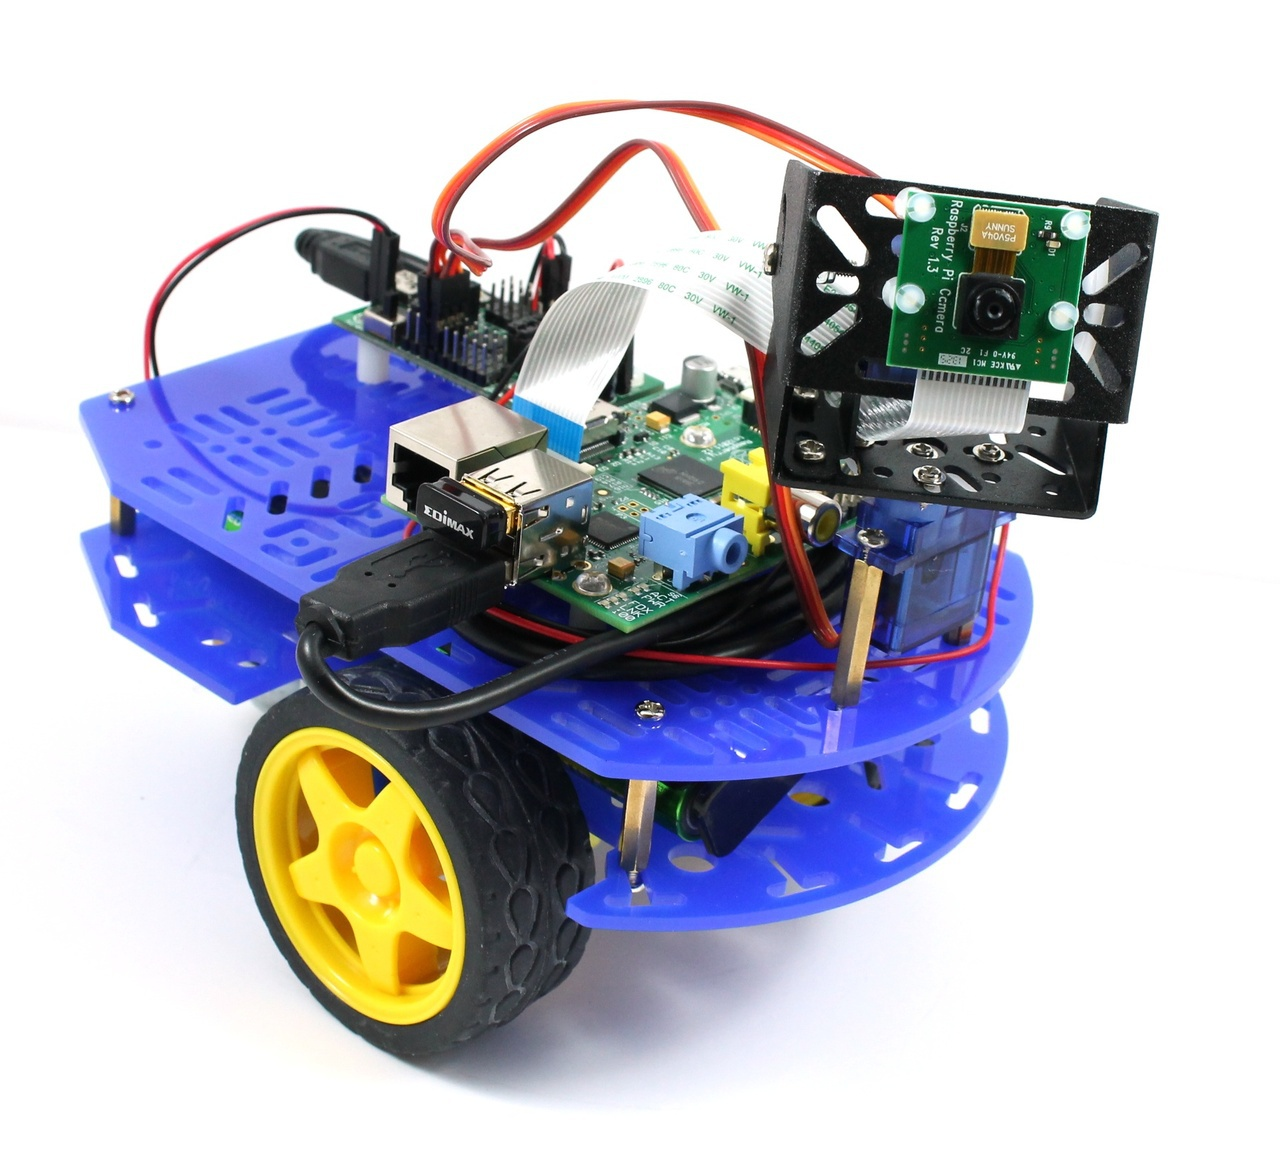
\includegraphics[scale=0.2]{images/kit.jpg}
\caption{Robot complet}
\end{figure}

\paragraph{Raspberry Pi} Nous avons donc utilisé deux modèles de Raspberry pi lors de notre projet : le Raspberry Pi B+ et le Raspberry Pi 2. 
Bien que visuellement, ces deux modèles se ressemblent très fort, leurs caractéristiques sont différentes :

\begin{tabular}{l|p{4.5 cm}|p{4.5 cm}}
 & Modèle B+ & Modèle 2 \\ 
\hline 
Mémoire RAM & 512 Mo & 1 Go \\ 
Processeur & ARMv6 & ARMv7 (4 coeurs) \\
Fréquence du processeur & 700 MHz & 900 MHz \\
Mémoire de stockage & MicroSD & MicroSD \\
Ports & 4 USB 2.0, HDMI, RJ45 \newline Jack (3.5mm), 40 broches GPIO & 4 USB 2.0, HDMI, RJ45, Jack (3.5mm), 40 broches GPIO \\
Consommation & 600 mA, 3.5 W & 600 mA, 3.5 W \\
Prix & environ 30 \euro & environ 40 \euro \\
Système d'exploitation & Linux & Linux, ou Windows 10
\end{tabular}

\begin{figure}[htbp]
\begin{minipage}[c]{.45\linewidth}
\begin{center}
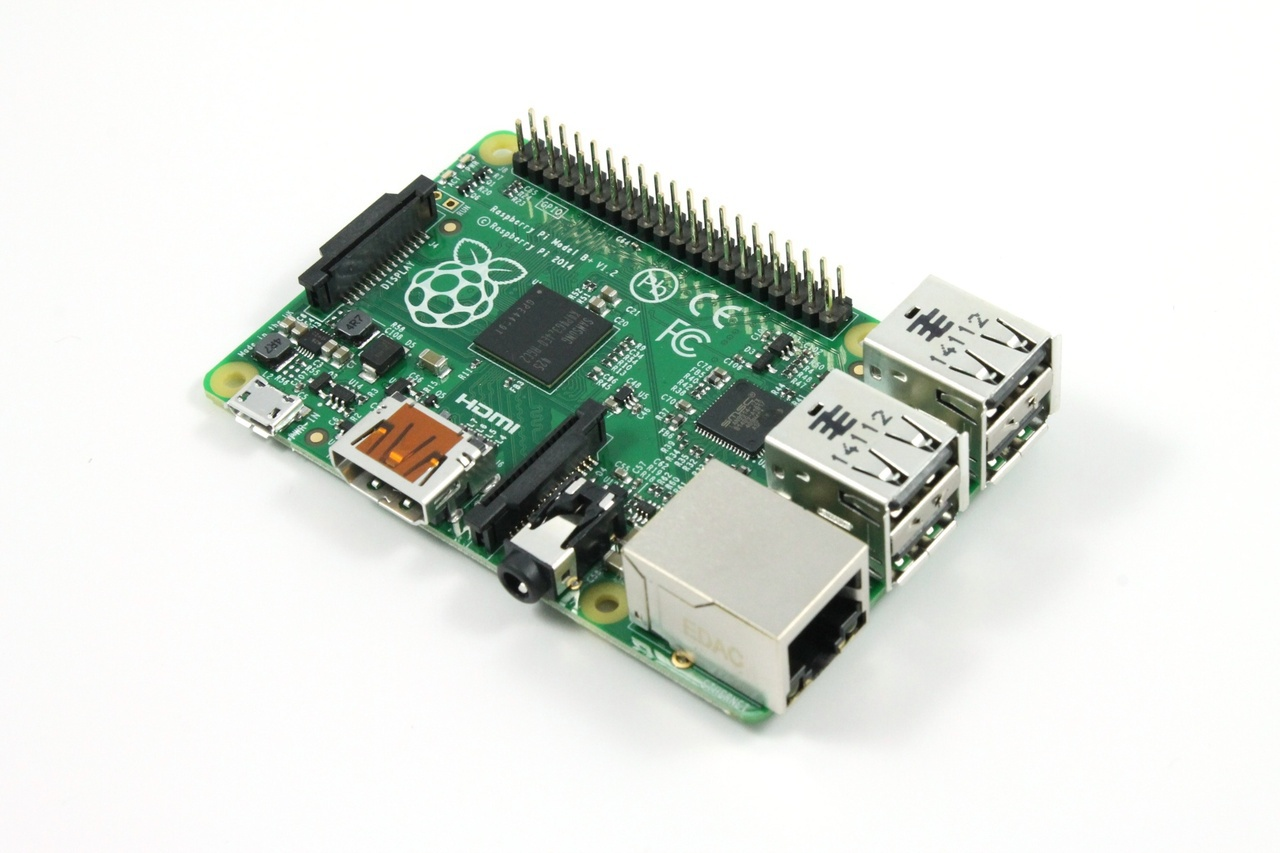
\includegraphics[scale=0.2]{images/modelB+.jpg}
\caption{Raspberry Pi B+}
%\label{}
\end{center}
\end{minipage}
\hfill
\begin{minipage}[c]{.45\linewidth}
\begin{center}
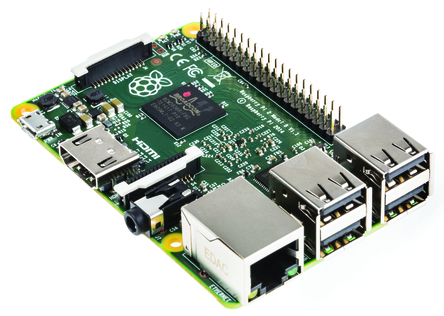
\includegraphics[scale=0.4]{images/model2.jpg}
\caption{Raspberry Pi 2}
%\label{}
\end{center}
\end{minipage}
\end{figure}

\paragraph{Arduino} C'est la carte Arduino qui fait le lien entre le Raspberry et les moteurs. Nous avons testé deux modèles différents :

\begin{tabular}{l|p{4.5 cm}|p{4.5 cm}}
 & Dagu mini driver & Dagu mini driver MKII \\ 
\hline 
Processeur & ATMega8A & ATMega328P \\
Fréquence du processeur & 16 MHz & 16 MHz \\
Prix & environ 10 \euro & environ 12 \euro \\
\end{tabular}

\begin{figure}[htbp]
\begin{minipage}[c]{.45\linewidth}
\begin{center}
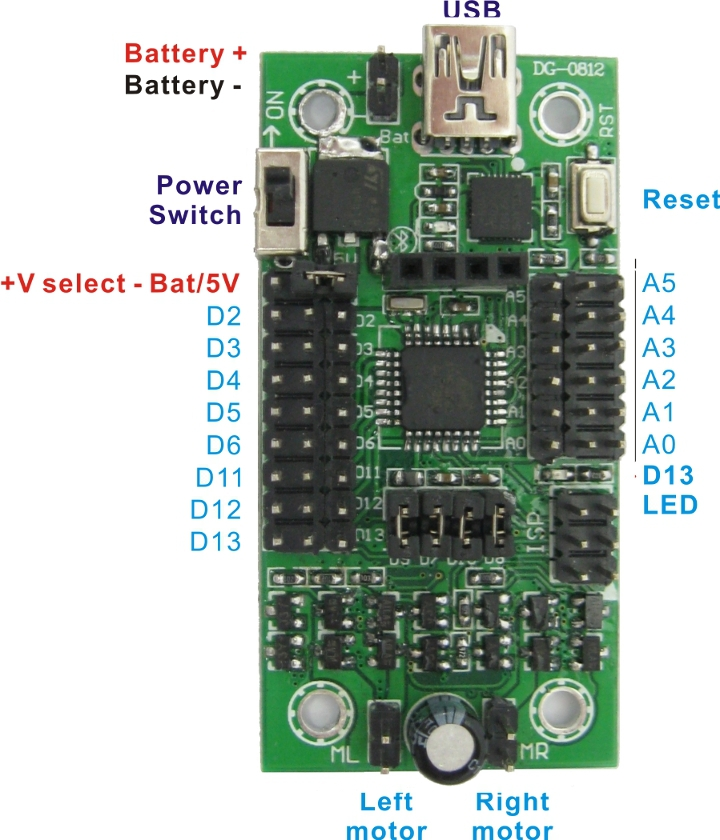
\includegraphics[scale=0.5]{images/mini_driver.jpg}
\caption{Dagu mini driver}
%\label{}
\end{center}
\end{minipage}
\hfill
\begin{minipage}[c]{.45\linewidth}
\begin{center}
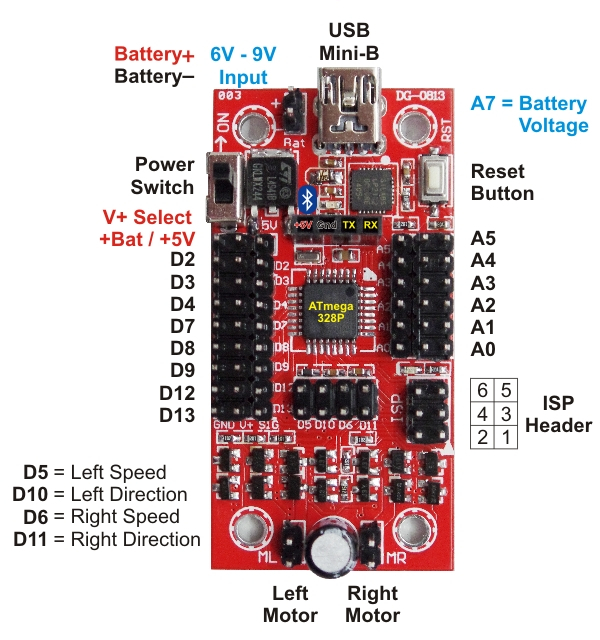
\includegraphics[scale=1]{images/Mini_Driver_MkII.jpg}
\caption{Dagu mini driver MKII}
%\label{}
\end{center}
\end{minipage}
\end{figure}

%\chapter{Software}
%
%%Trouver un autre titre !!!
%
%%Ici expliquer le principe des signaux PWM, des sockets, du multi-thread (même si pas utilisé... Parler des pistes envisagées)
%
%%Captures d'écran
%
%Lors de la réalisation du projet, nous avons envisagé plusieurs pistes pour contrôler le robot. 
%
%\section{Signaux PWM}
%
%Pour contrôler les moteurs, nous pouvons utiliser les signaux PWM (\textit{Pulse Width Modulation}) : il s'agit d'ondes carrées périodiques. 
%
%Pour chaque période, on envoie une tension continue de 5 volts (qui correspond à la tension de base du Raspberry Pi, délivrée sur les ports GPIO) pendant une fraction de la période seulement. La tension « perçue » par le moteur est directement proportionnelle à cette fraction. Si cette fraction vaut par exemple 60 \%, le moteur tournera comme si on envoyait 3 V, donc à 60 \% de son régime maximum, si sa tension nominale est de 5 V. 

\chapter{Implémentation}

\section{Le premier robot}

Nous avions , dans un premiers temps, travaillé avec le Raspberry pi B+ et un contrôleur DC (DRV8833) pouvant gérer deux moteurs (1.2 A , 2.7-10.8 V ). Cette solution, peut couteuse, nous a permis de travailler avec les pins GPIO du Raspberry.

Nos moteurs fonctionnaient avec une tension de 5 V, et étaient directement alimentés par ces pins. Nous avons beaucoup travaillé sur la partie électronique afin d'assembler au mieux un robot. Nous avions d'abord pensé implémenter directement dans le code l'envoi de signaux PWM dans les ports GPIO, avec une boucle dans le programme qui se répète toutes les 50 millisecondes et qui, selon les commandes envoyées, permet de faire avancer, tourner ou reculer le robot.

Les signaux PWM (Pulse Width Modulation) sont une technique qui nous permet d'obtenir une réponse analogique à partir d'un système fonctionnant en tout ou rien (système discret). Ce sont donc des ondes carrées dont le rapport de la largeur sur chaque période nous donne, dans ce cas-ci, la valeur de notre vitesse.
La largeur de pulsation correspond au laps de temps au cours duquel le système a la valeur 1 (5 V). Cette largeur rapportée sur l'entièreté de la période, nous donne le pourcentage d'activité, le Duty Cycle.

\begin{figure}[hf!]
\center
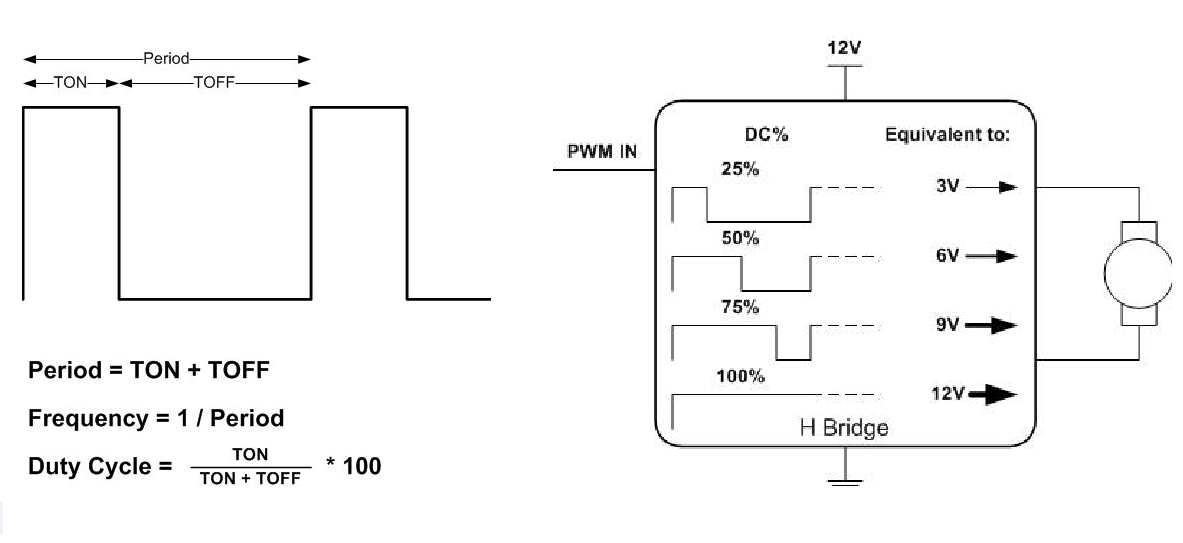
\includegraphics[scale=0.4]{images/PWM/totzal.png}
\caption{Principe des signaux PWM}
\end{figure}

Mais dans nos recherches, nous nous sommes aperçus que des librairies existaient déjà, et permettaient d'envoyer des signaux avec une seule commande, qui prenaient comme paramètre la vitesse relative des moteurs (100\% pour faire tourner le moteur à pleine vitesse vers l'avant, par exemple) 

Néanmoins, la qualité du matériel en notre possession n'était pas optimale : nous n'arrivions pas a fixer correctement les roues sur les axes des moteurs, et nous avons grillé le contrôleur DC lors de nos manipulations.

\begin{figure}[hf!]
\center
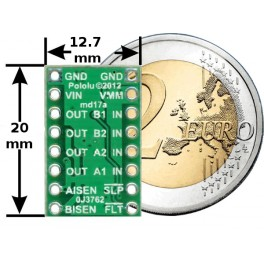
\includegraphics[scale=0.5]{images/y.jpg}
\caption{Contrôleur DRV8833}
\end{figure}

Nous avons réalisé à ce moment l'importance d'une bonne organisation de notre travail : nous avons opté pour une réalisation du projet étape par étape : c'est-à-dire que pour chaque chose à faire, nous la découpons en petites tâches "plus simples". Cette méthode présente deux avantages : nous voyons notre progression, car chaque étape est un pas vers la solution définitive, et si nous rencontrons un problème, nous pouvons revenir à une étape antérieure que nous savons fonctionnelle.

\section{Construction du second robot}

%Nous avons donc pris l'initiative de changer pour un kit qui nous permettrait de gagner du temps sur la partie électronique en utilisant une carte Arduino pour commander les moteurs, et surtout qui est  ayant des roues et un chassis adapté à nos envies.
Nous avons donc pris l'initiative de changer pour un kit qui nous permet d'avoir des composants compatibles entre eux, et de meilleure qualité.
%Les servo-moteurs étant géré par le raspberry afin de pouvoir jouer avec la caméra.
Les moteurs sont donc directement relié aux pins de la carte Arduino, elle-même reliée au Raspberry avec un câble USB.
L'ensemble du matériel utilisé est décrit en détail au chapitre \ref{Matériel}. La carte Arduino sert à rajouter une couche d'abstraction. Concrètement, cela permet de ne gérer que de la communication sur le Raspberry. Le contrôle des moteurs est géré par la carte Arduino. En travaillant comme cela, nous ne devons plus gérer la partie électronique (génération de signaux PWM, ...).

\subsection{Communication entre un PC et un Raspberry Pi}

Pour notre robot, la création d'une connexion Socket entre un PC et un Raspberry était nécessaire.

La première étape est de créer une connexion entre un PC et ce même PC. Nous avons trouvé plusieurs exemples sur internet qui fonctionnent. Mais nous avons voulu aller plus loin pour cette étape : 

\begin{figure}[hf!]
\center
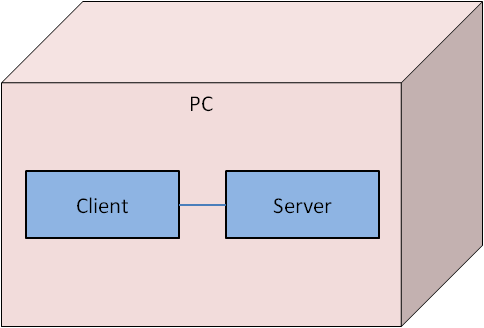
\includegraphics[scale=0.6]{images/Socket1.png}
\caption{Première étape}
\end{figure}

\begin{itemize}
\item Ne pas envoyer une chaîne de caractère directement du code, mais la demander à l'utilisateur.
\item Traiter la chaîne reçue sur l'autre programme, simplement l'afficher, afficher le premier caractère, ou si nous envoyons un nombre (envoyé sous forme de chaîne), récupérer ce nombre et effectuer une opération mathématique simple.
\item Envoyer une chaîne (n'importe quoi, cela n'a pas d'importance), puis dès que l'autre programme reçoit cette chaîne, renvoyer une autre chaîne.
\item Sur le PC, gérer avec Python les dates.
\end{itemize}

\bigbreak

Ainsi avec quelques étapes "faciles", nous pouvons affirmer :

\bigbreak

\begin{itemize}
\item Nous savons ouvrir une connexion,
\item Nous pouvons envoyer n'importe quelle information "simple" (types de données courants),
\item Nous savons la récupérer et la traiter de l'autre coté,
\item Nous savons estimer le temps que ça prend pour l'envoi (lors de nos tests, l'aller-retour prenait environ 0.7 secondes).
\item Nous savons comment fonctionne le code, car au lieu de recopier bêtement d'internet, nous l'avons modifié en cherchant à comprendre son fonctionnement.
\end{itemize}

\bigbreak

Ensuite, nous avons répété les mêmes processus entre un PC (sous Windows) et une machine virtuelle (sous Debian). Ces étapes sont normalement immédiates, puisque tous les codes ont déjà été écrits à l'étape précédente.

\begin{figure}[hf!]
\center
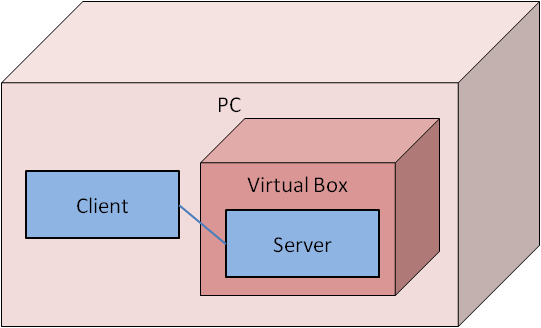
\includegraphics[scale=0.6]{images/Socket2.png}
\caption{Deuxième étape}
\end{figure}

\bigbreak

Enfin, nous avons refait la même chose entre le PC et le Raspberry. Nous avons dès lors atteint notre objectif, à savoir envoyer des instructions depuis le PC, vers le Raspberry.

\begin{figure}[hf!]
\center
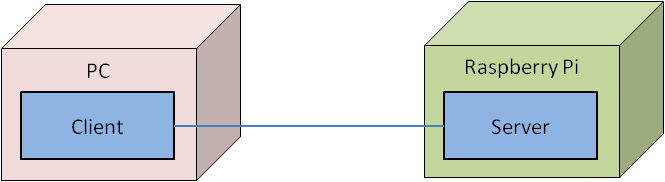
\includegraphics[scale=0.6]{images/Socket3.png}
\caption{Troisième étape}
\end{figure}

\subsection{Caméra}

L'une des fonctionnalités principales du robot est de filmer et de renvoyer l'image en temps réel vers l'utilisateur.

Nous avons utilisé une webcam, branchée sur un des ports USB du Raspberry. Le programme \textit{Motion} permettant alors d'envoyer l'image sur le réseau. L'utilisateur peut alors voir ces images, en entrant l'adresse IP du Raspberry, suivie du numéro du port. Nous avons configuré \textit{Motion} pour qu'il envoie sur le port 8081. L'adresse à entrer sur le navigateur est :

\begin{verbatimtab}[3]
192.168.1.50:8081
\end{verbatimtab}

Sur le kit que nous utilisons, un emplacement est prévu pour la picaméra, qui se connecte au Raspberry sur le port CSI (Camera Serial Interface)

\begin{figure}[hf!]
\center
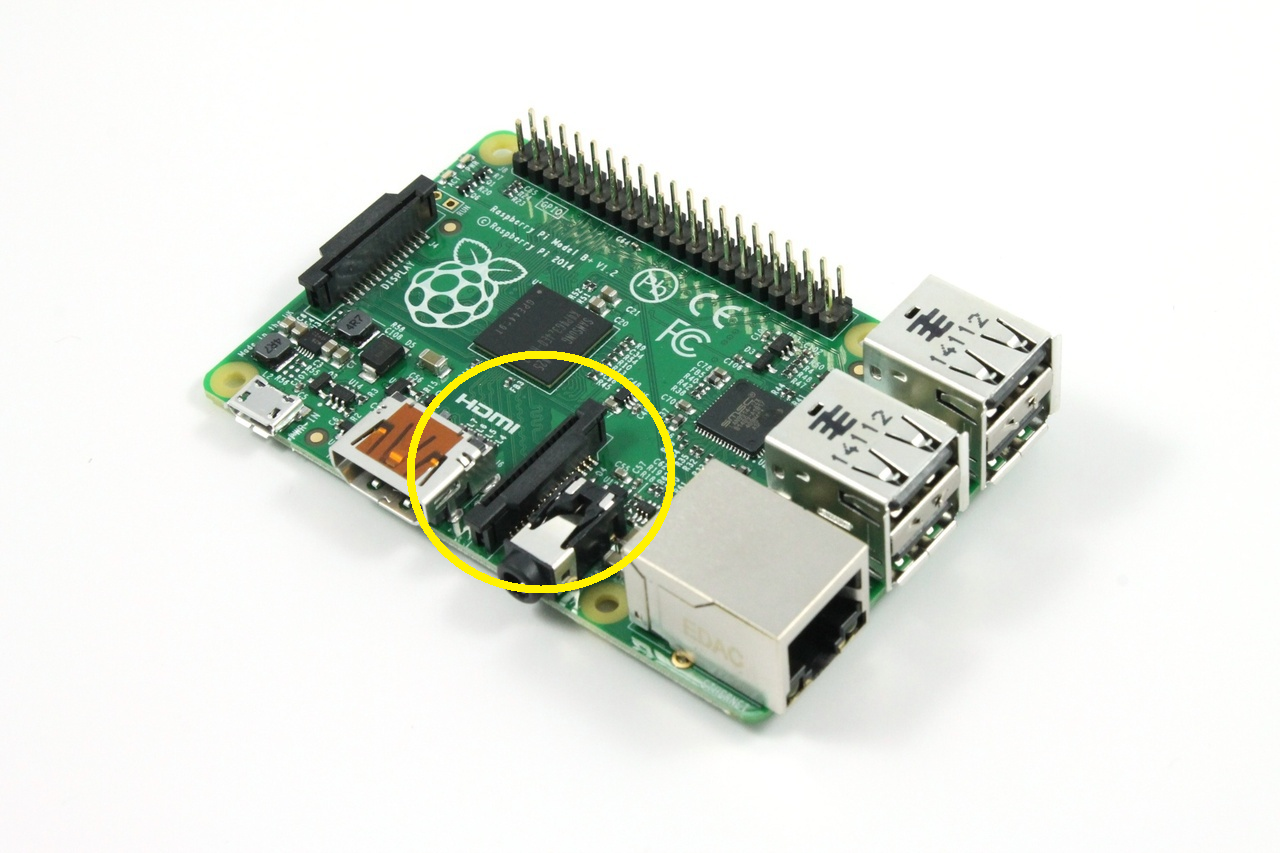
\includegraphics[scale=0.2]{images/portCSI.png}
\caption{Port CSI sur le Raspberry}
\end{figure}

Cette caméra présente toutefois un inconvénient : la nappe de câbles est trop courte, et si nous faisons faire des mouvements trop larges à la caméra (par exemple regarder à 90 degrés sur la gauche ou la droite), la nappe se détache du port.

Puisque nous ne savons pas remplacer la nappe, nous avons inclus dans le programme \textit{ControlMotors.ino} une limite d'angle de 45 degrés à gauche et à droite par rapport à l'avant du robot.

\chapter{Organisation}

\begin{figure}[hf!]
\center
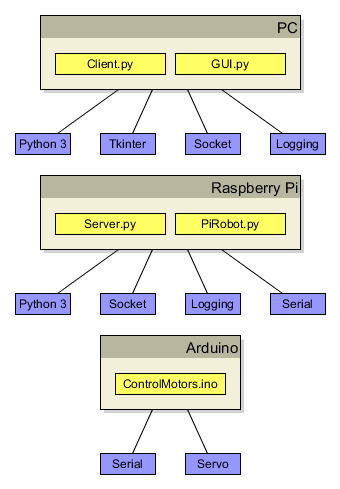
\includegraphics[scale=0.6]{images/GraphLogiciel.png}
\caption{Logiciel}
\end{figure}

Notre code est divisé en trois parties :

\bigbreak

\begin{itemize}
\item La partie Client, qui se trouve sur un PC (sous Windows, Linux, ...),
\item La partie Serveur, qui se trouve sur le Raspberry Pi,
\item La partie Contrôle, qui se trouve sur la carte Arduino.
\end{itemize}

\section{PC}

\paragraph{Client.py} sert à communiquer avec le Raspberry Pi. C'est dans ce fichier que sont récupérées toutes les requêtes de l'utilisateur, lorsqu'il appuie sur un bouton, par exemple. A chaque fois qu'un bouton est poussé, une instruction est envoyée. Lorsque le bouton est relâché, une instruction \verb=Stop= est envoyée.

\paragraph{GUI.py} sert à tracer l'interface graphique. Nous avons voulu créer des fonctions dans ce fichier et les lier directement au bouton comme ci-après :

\begin{verbatimtab}[3]
buttonstop = Button(frameRoot, text="STOP", command=buttonstopclick)
\end{verbatimtab}

Mais cela a entraîné des erreurs de références circulaires (car \textit{Client.py} dépend de \textit{GUI.py} et \textit{GUI.py} dépend de \textit{Client.py}). Nous avons résolu ce problème en ne donnant pas de fonction au bouton. Dans \textit{Client.py}, nous donnons explicitement la commande suivante :

\begin{verbatimtab}[3]
GUI.buttonstop.bind("<Button-1>", buttonstopclick)
\end{verbatimtab}

Cette seconde option présente deux avantages : on peut choisir le type d'événement à associer (bouton cliqué ou relâché, ...), et on peut aussi supprimer ce lien (avec la commande \verb=unbind=).

\begin{figure}[hf!]
\center
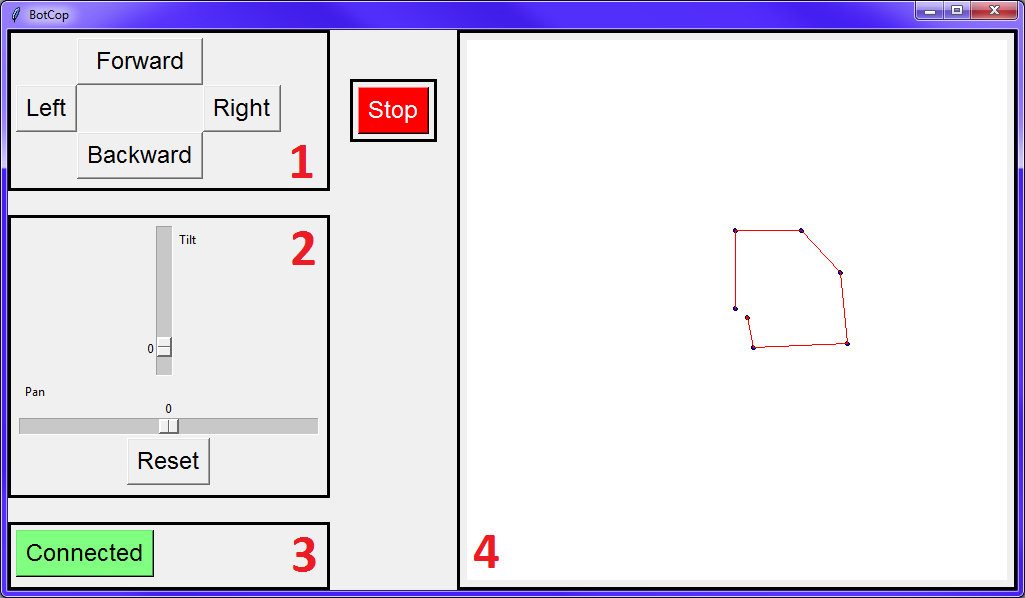
\includegraphics[scale=0.5]{images/Screen/Client2.png}
\caption{Interface graphique}
\end{figure}

L'interface est divisée en quatre zones, ou \textit{frames} :

\begin{itemize}
\item[1] Contrôle du robot, pour le déplacer. Le robot continuera à avancer/tourner tant que le bouton est enfoncé, et s'arrête dès que le bouton est relâché.
\item[2] Contrôle de la caméra, pour commander sa direction. Le bouton \verb=Reset= permet de remettre la caméra à son état initial, c'est-à-dire regarder droit devant le robot, à l'horizontale.
\item[3] Bouton de connexion. Tant que la connexion avec le Raspberry n'est pas établie, ce bouton restera rouge, et les autres boutons seront désactivés. Une fois que la connexion est établie, le bouton devient vert, et les autres boutons deviennent actifs.
\item[4] Visualisation du trajet. Chaque déplacement du robot peut être vu graphiquement sur cette zone. Pour réinitialiser le graphique, double-cliquez dessus.
\end{itemize}

\section{Raspberry Pi}

\paragraph{Server.py} est le programme qui tourne sur le Raspberry Pi. Son but est de recevoir les messages (depuis \textit{Client.py}, sur le PC) et de les interpréter pour envoyer des instructions au robot.

\paragraph{PiRobot.py} est une classe qui contient toutes les fonctions d'envoi de commandes au robot, ainsi quand \textit{Server.py} reçoit un message, il n'a qu'à appeler la bonne fonction (par exemple la fonction \verb=Stop=, qui envoie une commande au robot pour arrêter les moteurs).

A chaque instruction reçue, une nouvelle chaîne de caractère est crée. Elle se présente de la manière suivante :

\begin{verbatimtab}[3]
F180F180090020
\end{verbatimtab}

On peut la décomposer en quatre parties :

\begin{verbatimtab}[3]
F180 F180 090 020
\end{verbatimtab}

Les deux premières parties sont les instructions pour les moteurs (le gauche puis le droit). La lettre (\verb=F= ou \verb=B=) indique le sens (AVANT ou ARRIÈRE), et les trois chiffres suivants indiquent la vitesse relative (255 pour 100\% de la vitesse).

La troisième partie donne l'angle horizontal de la de la caméra (PAN). Par exemple \verb=090= sert à orienter la caméra droit devant le robot.

La quatrième partie donne l'angle vertical de la caméra (TILT).

Enfin, cela n'est pas indiqué, mais la chaîne se termine par un caractère \verb=\newline=, pour que le programme \textit{ControlMotors.ino} sache que la chaîne est terminée. 

\section{Arduino}

\paragraph{ControlMotors.ino} reçoit la chaine d'instructions depuis le Raspberry, et la découpe pour envoyer les instructions à chaque moteur. Cette action est répétée à chaque fois qu'un caractère \verb=\newline= est reçu.

\section{Informations supplémentaires}

\paragraph{Python 3} est la version de l'interpréteur utilisé. Nous précisons ce détail, car certaines fonctionnalités que nous utilisons ne portent pas les mêmes noms dans d'autres versions de Python, ou n'existent tout simplement pas. Sur le Raspberry, c'est la version 3.4, tandis que sur le PC, c'est la version 3.2.3. Il ne faut pas utiliser Python 2.7, car la compatibilité des programmes n'est pas assurée.

\paragraph{Tkinter} sert à tracer l'interface graphique. Il permet d'organiser assez facilement les éléments dans la fenêtre graphique.

\paragraph{Socket} permet d'ouvrir une connexion entre une machine hôte (appelée Serveur) et une ou plusieurs machines (appelées Clients). Une fois la connexion établie, les commandes \verb=send= et \verb=recv= permettent d'échanger des données.

\paragraph{Serial} permet d'ouvrir une connexion entre la carte Arduino et le Raspberry. La carte Arduino va se mettre à l'écoute sur un port choisi par l'utilisateur (port \verb=\ttyUSB0=). 

\paragraph{Logging} sert à protocoler des informations, en les stockant dans un fichier \text{.log}. Par exemple, la commande suivante est appelée dans la fonction \verb=buttonstopclick= :

\begin{verbatimtab}[3]
logging.debug('Button STOP click')
\end{verbatimtab}

Dans le fichier \text{.log}, nous verrons cette ligne apparaître :

\begin{verbatimtab}[3]
2015-07-28 18:06:08,051 root	DEBUG	Button STOP click
\end{verbatimtab}

C'est une alternative au \verb=print('Button STOP click')=, et qui permet de sauvegarder les actions faites lors de l'exécution d'un programme, même s'il est arrêté pour quelque raison que ce soit.

\paragraph{Github} est un système de contrôle de révision, et peut être utilisé pour plusieurs choses :

\begin{itemize}
\item Il permet d'enregistrer plusieurs versions d'un code, en montrant qui l'a mis en ligne, quand cela a été fait, et les différences avec la version précédente. C'est utile si nous nous rendons compte que les modifications apportées à un code rend celui-ci inutilisable, en permettant de retélécharger un code que nous savons fonctionnel. Sur la figure \ref{GitHub}, on voit que Sero17 (c'est le pseudo de Raphaël) a modifié le fichier \url{ClientGUI\GUI.py} il y a dix jours.
\item Il permet aussi de garder une copie des codes. Si l'ordinateur ou le Raspberry rencontre un problème, le code est sauvegardé.

\begin{figure}[hf!]
\center
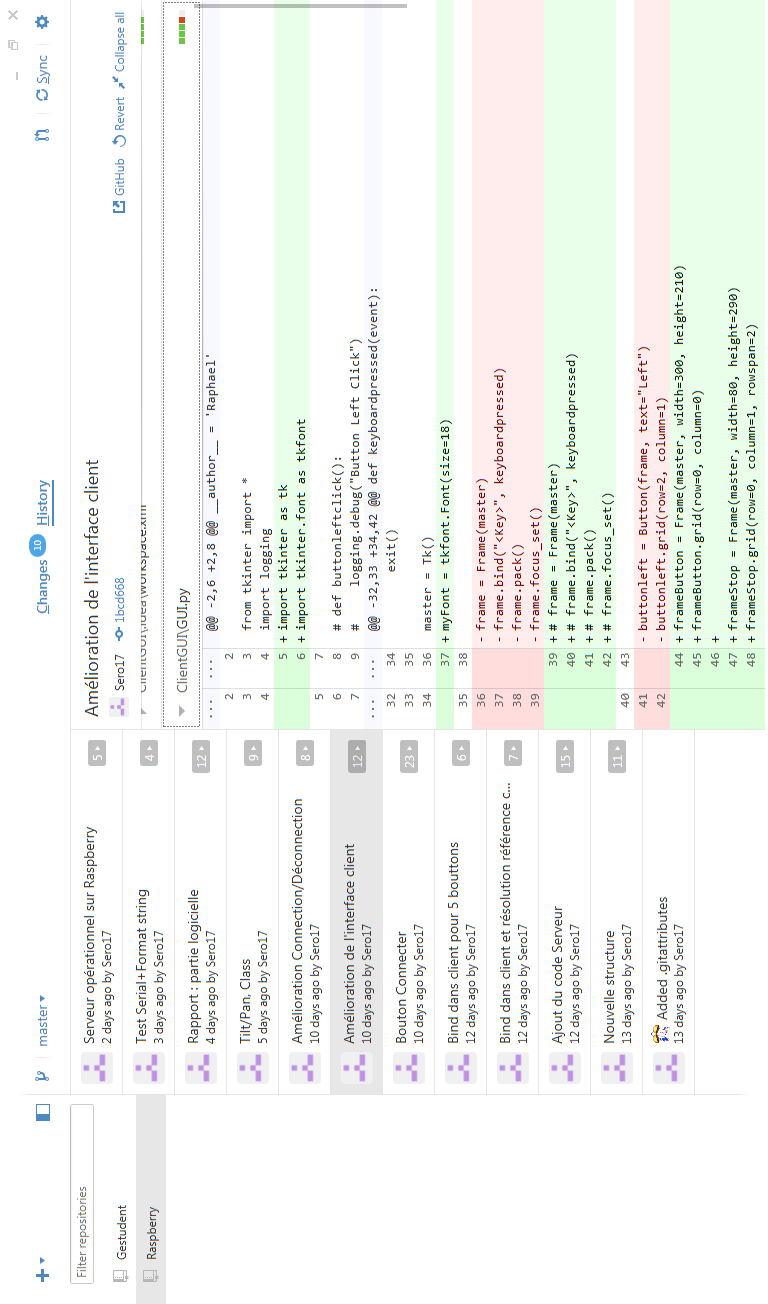
\includegraphics[scale=0.7]{images/GitHub.png}
\caption{Interface de GitHub sous Windows}
\label{GitHub}
\end{figure}

\end{itemize}

\chapter{Le programme en action !}

Pour contrôler le robot, il faut démarrer les programmes dans le bon ordre. Voici la marche à suivre :

\paragraph{Arduino} La première chose à faire est de télécharger le code sur la carte Arduino. Pour cela, démarrez l'IDE Arduino, et ouvrez le fichier .ino que vous voulez mettre sur la carte.

Dans \verb=Outils=, sélectionnez le modèle de carte (\verb=Arduino Nano w/ATmega328=), le port (\verb=ttyUSB0=) et le programmeur (\verb=AVRISP mkII=).

Vérifiez le code, et téléversez-le sur la carte.

Notez que la carte Arduino peut garder en mémoire un programme, même si elle est mise hors tension.

\paragraph{Raspberry Pi} Il faut démarrer le programme \textit{Server.py} sur le Raspberry. Bien sur, on peut connecter un écran, un clavier et une souris. Dans ce cas, ouvrez un terminal, et allez dans le dossier ou se trouve le programme. Par exemple, si le programme se trouve dans le dossier \textit{ServerRobot}, qui se trouve sur le bureau, entrez :

\begin{verbatimtab}[3]
cd Desktop/ServerRobot/
\end{verbatimtab}

Une fois dans le bon dossier, démarrez le programme avec :

\begin{verbatimtab}[3]
python3 Server.py
\end{verbatimtab}

Ce n'est pas très intéressant d'avoir un robot relié à un écran avec un câble HDMI. On peut se connecter à distance au Raspberry en utilisant Putty\footnote{Téléchargez Putty sur \url{http://www.chiark.greenend.org.uk/~sgtatham/putty/download.html}}. Introduisez l'adresse IP du Raspberry, le numéro de port (22), et le type de connexion (SSH). Lorsque la connexion sera établie, entrez l'identifiant \verb=pi= et le mot de passe \verb=raspberry=. Ensuite, il suffit de démarrer le programme comme décrit ci-dessus.

\begin{figure}[hf!]
\center
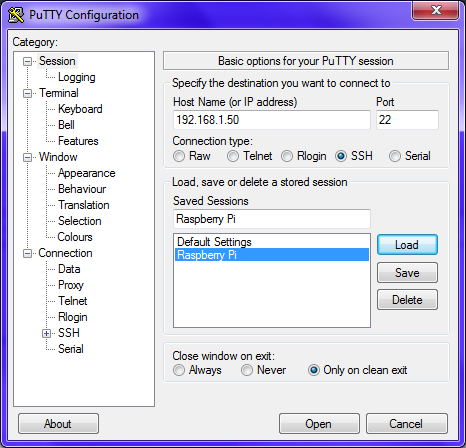
\includegraphics[scale=0.7]{images/Screen/Putty.png}
\caption{Configuraton de Putty}
\end{figure}

\paragraph{PC} Enfin, démarrez sur le PC le programme \textit{Client.py}, et appuyez sur le bouton \verb=Connect= en bas à gauche.

\chapter{Conclusion}

Ce projet nous a permis de découvrir et d'apprendre plusieurs choses : la programmation sur carte, la possibilité de contrôler un moteur à partir d'un programme, le langage Python, ... Mais aussi à organiser un programme quand celui-ci est en plusieurs parties. Il faut en effet avoir une vision globale de l'architecture logicielle pour pouvoir s'y retrouver.

Gérer un timing a été le plus difficile dans ce projet, notamment à cause de nombreux imprévus (matériel défectueux, ...). De même, c'était pour nous la première fois que nous avons du travailler en équipe sur un projet d'informatique.

Dans ce projet, nous avons surtout été limités par le matériel. Nous avons perdu beaucoup de temps pour nous rendre compte qu'un des composants ne fonctionne plus (cela nous est arrivé plusieurs fois). Un autre problème que nous avons eu est que le deuxième modèle de carte Arduino demande une tension supérieure à ce que la batterie peut fournir.

Pour encore améliorer notre robot, on pourrait imaginer rajouter des fonctonnalités pour la caméra : possibilité d'enregistrer une image ou un film, et éventuellement de déclencher cet enregistrement si un mouvement quelconque est détecté. On pourrait ajouter une lampe (pour que le robot puisse filmer dans le noir).

\appendix

\chapter{Procédure d'installation}

\section{Installation de Raspbian sur le Raspberry Pi}

Voici la procédure à suivre pour installer Raspbian sur le Raspberry :

\begin{itemize}
\item Téléchargez NOOBS sur \,\url{https://www.raspberrypi.org/downloads/}, et extrayez les fichiers du zip.

\item Formatez la carte SD (avec \,\url{https://www.sdcard.org/downloads/formatter_4/}). Sélectionnez la carte SD et dans les options choisissez \textit{FORMAT SIZE ADJUSTMENT ON}, puis cliquez sur \verb=Format=.

\item Copiez les fichiers extraits de NOOBS sur la carte SD, puis éjectez la carte et insérez-la dans le Raspberry Pi.

\item Connectez le Raspberry à un écran avec un câble HDMI, et connectez aussi un clavier et une souris sur les ports USB (un récepteur sans fil convient aussi).

\item Alimentez le Raspberry. Attention il est déconseillé de brancher/débrancher des câbles lorsque le Raspberry est sous tension. Si vous souhaitez changer l'écran ou un autre périphérique, éteignez d'abord le Raspberry et débranchez-le.

\item Sélectionnez Rasbian comme OS et la langue, ainsi que la configuration du clavier, et cliquez sur \textit{Installer}.

\item Après l'installation (compter environ 25 minutes), redémarrez le Raspberry Pi.

\item Dans les options proposées, choisissez \textit{Enable Boot to Desktop/Scratch}, et \textit{Desktop Log in as user 'pi'}. Ensuite dans \textit{Advanced Options}, choisissez \textit{SSH}, et \textit{Enable}. Allez sur \textit{Finish} (avec Tabulation) et redémarrez le Raspberry.

\item Si vous utilisez un écran avec un câble VGA et un adaptateur, il faut modifier \url{\boot\config.txt}. Il faut décommenter ou ajouter les lignes suivantes : 
\begin{verbatimtab}[3]
hdmi_force_hotplug=1
hdmi_group=2
hdmi_mode=69
hdmi_drive=2
\end{verbatimtab}
Le numéro 69 correspond à une résolution d'écran de 1920x1200, et une fréquence de 60 hz. Pour voir quel numéro correspond, voir \url{https://www.raspberrypi.org/documentation/configuration/config-txt.md}\, .

\item Configurez le WiFi (voir section suivante), et mettez à jour le système en entrant ces deux commandes :

\bigbreak
\begin{verbatimtab}[3]
sudo apt-get update
sudo apt-get upgrade
\end{verbatimtab}
\bigbreak

\end{itemize}



\section{Configurer le WiFi sur le Raspberry Pi}

Nous allons configurer le Raspberry pour se connecter au routeur, et lui assigner une IP fixe.

\begin{itemize}
\item Lorsque le Raspberry est hors tension, insérez la clé WiFi dans un port USB.
%\item Dans un terminal, entrez la commande \,\verb=ifconfig= pour récupérer ceci :
%
%\bigbreak
%\begin{verbatimtab}[3]
%wlan0	Link encap:Ethernet	HWaddr c4:a8:1d:7c:0b:60
%inet adr:192.168.1.104	Bcast:192.168.1.255	Masque:255.255.255.0
%\end{verbatimtab}
%\bigbreak
%
%\item Entrez ensuite \,\verb=sudo route -n=  :
%
%\bigbreak
%\begin{tabular}{lll}
%\verb=Destination= & \verb=Passerelle= & \verb=Genmask= \\ 
%\verb=0.0.0.0= & \verb=192.168.1.1= & \verb=0.0.0.0= \\ 
%\verb=192.168.1.0= & \verb=0.0.0.0= & \verb=255.255.255.0=\\ 
%\end{tabular}
%\bigbreak

\item Toutes les informations concernant le réseau peuvent être retrouvées grâce à un autre appareil connecté à ce réseau : entrez dans un terminal ces deux commandes :

\bigbreak
\begin{verbatimtab}[3]
sudo route -n
ifconfig
\end{verbatimtab}
\bigbreak

\item On édite un premier fichier de configuration : entrez cette commande : 

\bigbreak
\begin{verbatimtab}[3]
sudo nano /etc/wpa_supplicant/wpa_supplicant.conf
\end{verbatimtab}
\bigbreak

Ajoutez les paramètres du réseau Wi-Fi, et sauvegardez :

\begin{verbatimtab}[3]
network={
	ssid="<SSID du réseau local>"
	psk="<Clé de sécurité>"
	proto=RSN
	key_mgmt=WPA-PSK
	paiwise=CCMP
	auth_alg=OPEN
}
\end{verbatimtab}

\item On édite un autre fichier : entrez cette commande : 

\bigbreak
\begin{verbatimtab}[3]
sudo nano /etc/network/interfaces
\end{verbatimtab}
\bigbreak

Ajoutez les paramètres du réseau Wi-Fi, et sauvegardez :

\bigbreak
\begin{verbatimtab}[3]
auto lo

iface lo inet loopback
iface eth0 inet dhcp

allow-hotplug wlan0
auto wlan0

iface wlan0 inet static
address 192.168.1.50
netmask 255.255.255.0
broadcast 192.168.1.255
gateway 192.168.1.1
wpa-conf /etc/wpa_supplicant/wpa_supplicant.conf
iface default inet dhcp
\end{verbatimtab}
\bigbreak

L'adresse 192.168.1.50 est l'adresse IP que j'ai choisie pour le Raspberry. Il faut choisir une adresse en dehors de la plage d'adresse réservée pour le dhcp.

\item Réinitialisez le réseau avec ces deux commandes, ou redémarrez le Raspberry.

\bigbreak
\begin{verbatimtab}[3]
sudo ifdown wlan0
sudo ifup wlan0
\end{verbatimtab}
\bigbreak
\end{itemize}

\chapter{Qui a fait quoi}

\section{Raphaël LEJEUNE}

Lors de ce projet, je me suis occupé de la partie logicielle : j'ai effectué les recherches suivantes : 

\paragraph{Configuration} Comment configurer le Raspberry pour qu'il puisse se connecter à internet. Il fallait aussi lui assigner une IP fixe, pour faciliter les communications avec la PC.

\paragraph{Communication} Comment envoyer des informations depuis le PC vers le Raspberry, et depuis le Raspberry vers la carte Arduino. Ces recherches incluent aussi la compréhension des exemples trouvés sur internet, dans le but d'avoir une meilleure maitrise des programmes que j'écris.

\paragraph{Interface} Comment créer une interface graphique en Python. Une fois Tkinter trouvé, le même travail de recherche, d'essais et de compréhension du fonctionnement du package a du être fait.

\paragraph{Caméra} J'ai aussi mené quelques recherches pour la caméra, et pour récupérer l'image via le réseau.

Après les travaux de recherche, j'ai écrit les trois programmes :

\paragraph{PC} L'interface graphique : j'ai agencé les boutons pour avoir une fenêtre aussi organisée et logique que possible. J'ai aussi décidé que les messages envoyés seraient du type "FORWARD" ou "STOP".

\paragraph{Raspberry} Le serveur : j'ai géré deux types de communication (Socket et Serial). J'ai placé tout ce qui concerne l'envoi vers la carte Arduino dans une classe séparée, tandis que dans le programme principal, j'ai utilisé le formatage de chaîne pour faciliter le travail sur la carte Arduino.

\paragraph{Arduino} Ici mon travail a surtout été de récupérer la chaîne reçue du Raspberry, de la découper pour pouvoir envoyer les instructions aux moteurs.

J'ai utilisé GitHub pour garder une trace de chaque étape que j'ai réalisée. Lors de la rédaction du rapport, j'ai rédigé toutes les parties consacrées au logiciel (organisation, procédures d'installation, ...)

\section{Maximilien POTTIEZ}

En ce qui me concerne , je me suis occupé de la recherche, de l'achat et du montage du matériel.
Je me suis intéressé à l'électronique du projet et à la manipulation de Linux.
J'ai appris à souder grâce à l'aide du service d'électronique. 
De plus, il a fallu s'intéresser et comprendre de nombreux concepts et outils tels que les signaux PWM et leur fonctionnement à travers les contrôleurs.
Le projet m'a permis de maitriser des éditeurs de texte comme vim ,le langage python et différentes de ses bibliothèques, de même que SSH et bien d'autres concepts utiles.
De nombreuses directions furent prises lors de la conception de ce projet et beaucoup de concept appris ne se retrouvent pas dans le produit final tel que l'utilisation d'opencv, pygame et autres.

\chapter{Sources}

Voici la liste des sites internet que nous avons consultés pour ce projet

\begin{itemize}
\item http://www.dawnrobotics.co.uk/dagu-arduino-mini-driver-board/
\item http://www.dawnrobotics.co.uk/dagu-arduino-mini-driver-mkii/
\item http://blog.dawnrobotics.co.uk/2013/11/getting-started-with-the-dagu-arduino-mini-driver-board/
\item http://blog.dawnrobotics.co.uk/2014/06/programming-raspberry-pi-robot-using-python-opencv/
\item http://www.dawnrobotics.co.uk/raspberry-pi-camera-robot-chassis-bundle/
\item http://blog.oscarliang.net/connect-raspberry-pi-and-arduino-usb-cable/
\item http://stackoverflow.com/questions/20107700/serial-receiving-from-arduino-to-raspberry-pi-with-pyserial-stops-after-a-while
\item https://www.raspberrypi.org/forums/viewtopic.php?t=50243\&p=389997
\item https://www.raspberrypi.org/documentation/configuration/wireless/wireless-cli.md
\item http://lifehacker.com/how-to-clone-your-raspberry-pi-sd-card-for-super-easy-r-1261113524
\item https://docs.python.org/3.2/library/socket.html
\item http://www.robot-maker.com/forum/tutorials/article/78-rcerda-un-robot-raspberry-pi-pour-100-120/
\item http://www.fred-j.org/?p=366
\item http://lea-linux.org/documentations/Raspberry\_Pi
\end{itemize}

\end{document}